\section{Einf"uhrung}
\label{sec:Einf"uhrung}
Gegenstand dieser Bachelorarbeit ist der Zusammenhang zwischen den Eigenwerten, der chromatischen Zahl und den Krauszzerlegungen eines Graphen. Die daf"ur ben"otigten Grundlagen werden wir in Kapitel 1 erarbeiten. 
\subsection{Graphen und Hypergraphen}
\label{ssec:graphenundhypergraphen}
Die in dieser Arbeit betrachteten Graphen und Hypergraphen sind endlich und haben weder Mehrfachkanten noch Schlingen. Bei den Bezeichnungen richten wir uns im Wesentlichen nach dem Buch von Diestel \cite{Diestel10} beziehungsweise dem Buch von Berge \cite{Berge01}. 
Mit $\N$ bezeichnen wir die Menge der positiven ganzen Zahlen und setzen $\N_{0} = \N \cup \{ 0 \}$. F"ur eine Menge $V$ sei die Menge $2^{V}$ die Potenzmenge von $V$ und $[V]^{p}$ mit $p\in\N_0$ die Menge der $p$-elementigen Teilmengen von $V$. 

Ein \DF{Hypergraph} $H$ ist ein Tupel von zwei Menge, $V(H)$ und $E(H)$. Dabei ist $V(H)$ endlich und $E(H)$ eine Teilmenge von $2^{V(H)}$ mit $|e| \geq 2$ f"ur alle $e\in E(H)$. Die Menge $V(H)$ hei{\ss}t dann \DF{Eckenmenge} von $H$ und ihre Elemente hei{\ss}en \DF{Ecken} von $H$. Die Menge $E(H)$ hei{\ss}t \DF{Kantenmenge} und ihre Elemente hei{\ss}en \DF{Kanten}. Ein Hypergraph hei{\ss}t \DF{linear}, falls zwei verschiedene Kanten h"ochstens eine Ecke gemeinsam haben. 
Ist $V(H) = \varnothing$, so nennen wir $H$ auch den \DF{leeren Graphen} und schreiben kurz $H=\varnothing$.

Sei $H$ ein Hypergraph. Die \DF{Ordnung} von $H$ ist die Anzahl der Ecken von $H$, geschrieben $|H|$. Eine Kante $e$ hei{\ss}t \DF{Hyperkante}, falls $|e| \geq 3$ ist und hei{\ss}t \DF{gew"ohnliche Kante}, falls $|e| =2$ ist. F"ur eine gew"ohnliche Kante $e=\{ u,v \}$ schreiben wir auch kurz $e=uv$ oder $e=vu$. 
Ist $E(H) \subseteq [V]^p$, so nennen wir $H$ \DF{$p$-uniform}. Ein \DF{Graph} ist ein $2$-uniformer Hypergraph, also ein Hypergraph in dem jede Kante gew"ohnlich ist. Eine Ecke $v$ ist \DF{inzident} mit einer Kante $e$, falls $v\in e$ gilt. F"ur eine Ecke $v$ von $H$ sei $E_{H}(v) = \set{ e\in E(H) }{ v\in e }$ die Menge aller mit $v$ inzidenten Kanten. Der \DF{Grad} einer Ecke $v$ ist $d_{H}(v) = |E_H(v)|$. 
Der \DF{Minimalgrad} (\DF{Maximalgrad}) sei definiert als der kleinste (gr"o{\ss}te) Grad einer Ecke von $H$ und wird mit $\delta(H)$ ($\Delta(H)$) bezeichnet. F"ur $H=\varnothing$ setzen wir $\delta(H) = \Delta(H) = 0$. Ist $\delta(H) = \Delta(H) = r$, so hei{\ss}t $H$ $r$-regul"ar. 

Ein \DF{Unterhypergraph} von $H$ ist ein Hypergraph $H'$ mit $V(H') \subseteq V(H)$ und $E(H') \subseteq E(H)$. Wir schreiben dann $H' \subseteq H$. Gilt zus"atzlich $H' \neq H$, so ist $H'$ ein \DF{echter Unterhypergraph}. Gibt es eine Menge $X \subseteq V(H)$, sodass  $V(H') = X$ und $E(H') = E(H) \cap 2^{X}$ gilt, so ist $H'$ ein \DF{induzierter Unterhypergraph} und wir schreiben $H'= H[X]$ oder $H' \unlhd H$.  
Ist $X\subseteq V(H)$, so bezeichne $H-X = H[V(H) \setminus X]$. Ist $X=\{ v \}$, so schreiben wir daf"ur auch $H-v$ statt $H-\{v\}$. Ist $F\subseteq 2^{V(H)}$ eine Menge, so sei $H-F$ der Hypergraph mit Eckenmenge $V(H)$ und Kantenmenge $E(H) \setminus F$ und $H+F$ der Hypergraph mit Eckenemenge $V(H)$ und Kantenmenge $E(H) \cup F$. Ist $F= \{ e \}$ so schreiben wir $H\pm e$ anstatt $H\pm  \{ e \}$. 

Eine Menge von Ecken $X\subseteq V(H)$ hei{\ss}t \DF{unabh"angige Menge} von $H$, falls $E(H[X]) = \varnothing$ gilt. Die \DF{Unabh"angigkeitszahl} $\alpha(H)$ ist die Ordnung der gr"o{\ss}ten unabh"anigegen Menge von $H$. Eine Menge von Ecken $X\subseteq V(H)$ hei{\ss}t \DF{Clique} von $H$, falls $H[X]$ alle gew"ohnlichen Kanten von $[X]^{2}$ enth"alt. Die \DF{Cliquenzahl} $\omega(H)$ ist die Ordnung der gr"o{\ss}ten Clique von $H$. 

Sind $H,H'$ zwei Hypergraphen, so hei�t eine bijektive Abbildung $f : V(H) \to V(H')$ \DF{Isomorphismus} zwischen $H$ und $H'$, falls f"ur alle Teilmengen $\{ v_1,v_2,\dots, v_p \}$ von Ecken von $V(H)$ gilt: $$ \{ v_1,v_2,\dots, v_p \} \text{ ist Kante von $H$} \Leftrightarrow \{ f(v_1),f(v_2),\dots, f(v_p) \} \text{ ist Kante von $H'$}.$$ Zwei Hypergraphen $H,H'$ hei�en \DF{isomorph}, falls es einen Isomorphismus zwischen
$H$ und $H'$ gibt. 

F"ur einen Graphen $G$ sei $\overline{G}$ der \DF{Komplementargraph} von $G$ mit $V(\overline{G}) = V(G)$ und $E(\overline{G}) = [V(G)]^{2}\setminus E(G)$.  
Ein Graph $G$ hei{\ss}t \DF{vollst"andiger Graph}, falls $E(G) = [V(G)]^{2}$ gilt. Ist $G$ ein vollst"andiger Graph der Ordnung $n$, so schreiben wir auch $G=K_n$. Man beachte hierbei, dass alle vollst"andigen Graphen der Ordnung $n$ isomorph sind. In diesem Sinne bezeichnen wir mit $C_n$ den \DF{Kreis} der Ordnung $n$ und mit $O_n$ den \DF{kantenlosen Graphen} der Ordnung $n$ (d.h. das Komplement von $K_n$). 
Ein Kreis $C_n$ hei�t \DF{gerade} beziehungsweise \DF{ungerade}, je nachdem ob seine Ordnung gerade beziehungsweise ungerade ist.

F"ur einen Hypergraphen $H$ ist $\omega(H)$ die gr"o{\ss}te Zahl $n$, sodass $H$ einen vollst"andigen Graphen der Ordnung $n$ als Untergraphen enth"alt, und $\alpha(H)$ ist die gr"o{\ss}te Zahl $n$, sodass $H$ den kantenlosen Graphen der Ordnung $n$ als induzierten Untergraphen enth"alt. 

\subsection{F"arbungen von Graphen und Hypergraphen}

Das \DF{F\"arbungsproblem} f\"ur Graphen ist ein klassischen Problem aus der Graphentheorie mit vielf\"altigen Anwendungen in der kombinatorischen Optimierung und anderen Teilgebieten der Mathematik. Beim  F\"arbungsproblem besteht die Aufgabe darin, die Ecken eines Graphen so zu f\"arben, dass durch eine Kante verbundene Ecken verschiedenen Farben erhalten. Dabei sollen nat\"urlich m\"oglichst wenige Farben verwendet werden.

Seien $G$ ein Graph $C$ eine Menge. Eine Abbildung $\varphi :V(G) \to C$ hei{\ss}t \DF{F"arbung} von $G$, falls f"ur alle Kanten $vw$ von $G$ gilt: $\varphi (v) \neq \varphi (w)$. Ist $|C| = k \in \N_0$, so hei{\ss}t $\varphi $ auch \DF{$k$-F"arbung}. Besitzt ein Graph $G$ eine $k$-F"arbung, so hei�t $G$ \DF{$k$-f"arbbar}.
Die kleinste nat"urliche Zahl $k$, f"ur die $G$ eine $k$-F"arbung besitzt, bezeichnen wir mit $\chi(G)$, der \DF{chromatischen Zahl} von $G$. 
Ist die chromatische Zahl von $G$ gleich $k$, so wird $G$ auch \DF{$k$-chromatisch} genannt.

Die Bestimmung der chromatischen Zahl eines Graphen ist ein {\sf NP}-schweres Optimierungsproblem, wie im Jahre 1972 von Karp \cite{Karp72} gezeigt wurde. Sei $\varphi $ eine F"arbung von $G$ und $H$ ein Untergraph von $G$. Dann ist $\varphi |_{V(H)}$ eine F"arbung von $H$. Folglich ist die chromatische Zahl ein monotoner Graphenparameter, d.h. $$ H\subseteq G \Rightarrow \chi(H) \leq \chi(G).$$
Au�erdem ist die chromatische Zahl subadditiv, d.h. sind $X,Y$ zwei Teilmengen von $V(G)$ mit $X\cup Y = V(G)$, so gilt $$\chi(G) \leq \chi(G[X])+ \chi(G[Y]).$$ 
Ist n"amlich $\chi(G[X]) = k$ und $\chi(G[Y])= \ell$, so erhalten wir eine $(k+\ell)$-F"arbung von $G$, indem wir zun"achst alle Ecken aus $X$ mit $k$ Farben f"arben, und dann die verbleibenden Ecken aus $Y\setminus X$ mit h"ochstens $\ell$ Farben f"arben.

Eine Abbildung $\varphi  :V(G) \to C$ ist genau dann eine F"arbung von $G$, wenn f"ur alle $c\in C$ das Urbild $\varphi ^{-1}(c)$ eine unabh"angige Menge in $G$ ist (d.h. keine zwei Ecken von $\varphi ^{-1}(c)$ sind durch eine Kante von $G$ verbunden). Diese Urbilder nennen wir \DF{Farbklassen}. Offensichtlich sind die Farbklassen disjunkt und haben h"ochstens $\alpha (G)$ Ecken. Daraus folgt, dass jede $k$-F"arbung von $G$ die Ungleichung $|G| \leq k \alpha(G)$ erf"ullt, und deswegen auch $|G| \leq \chi(G) \alpha(G)$ gilt. 

Da jede Ecke eine unabh"angige Menge ist, gilt $\chi(G) \leq |G|$. Damit gilt 
$$\chi(G) \geq |G|  \Leftrightarrow \chi(G) = |G| \Leftrightarrow \alpha(G) \leq 1 \Leftrightarrow G \text{ ist ein vollst"andiger Graph}$$
Insbesondere gilt somit f"ur $n\in \N_0$ : $\chi(K_n)  = n $. Da $\chi $ ein monotoner Graphenparameter ist, ist also 
$$\omega(G) \leq \chi(G).$$

Die chromatische Zahl des Graphen $G$ ist die kleinste Zahl $k$, f"ur die sich $V(G)$ in $k$ viele unabh"angige Mengen (die Farbklassen) zerlegen l"asst. Deswegen gilt $\chi(G) = 0$ nur, falls $V(G)\neq \varnothing$ ist, d.h. falls $G$ der leere Graph ist. Au�erdem ist $\chi(G) \leq 1$ genau dann, wenn $G$ keine Kanten hat, und $\chi(G) \leq 2$ gilt genau dann, wenn $G$ bipartit ist.
Nach dem Satz von K"onig \cite{Konig16} ist $G$ genau dann bipartit, wenn $G$ keinen Kreis ungerader Ordnung als Untergraphen besitzt. 

Nach Stockmeyer \cite{Stockmeyer73} ist f"ur jedes $k\geq 3$ das Entscheidungsproblem ob ein gegebener Graph $k$-f"arbbar ist {\sf NP}-vollst"andig. Es ist also nicht zu erwarten, dass sich Graphen mit chromatischer Zahl h"ochstens $k$ f"ur festes $k\geq 3$ einfach charakterisieren lassen.

Bei der Untersuchung des F"arbungsproblems f"ur Graphen erweisen sich die kritischen Graphen als ein n"utzliches Hilfsmittel. Dies liegt vor allem daran, dass sich F"arbungsprobleme f"ur Graphen oft auf entsprechende F"arbungsprobleme f"ur kritische Graphen zur"uckf"uhren lassen.
Ein Graph $G$ hei{\ss}t \DF{k-kritisch}, falls $\chi(G) = k$ ist und $\chi(H) < k$ f"ur alle echten induzierten Untergraphen $H$ von $G$ gilt. 

Entfernen wir aus einem Graphen $G$ eine Ecke oder Kante, so bleibt die chromatische Zahl gleich oder verringert sich um den Wert $1$, d.h. f"ur $t\in V(G) \cup E(G)$ gilt:
\begin{equation}
  \chi(G) -1 \leq \chi(G-t) \leq \chi(G).
  \label{eq:chiungl}
\end{equation}
Daraus erhalten wir den folgenden bekannten Satz, wonach die $(k-1)$-f"arbbaren Graphen durch verbotene $k$-kritische Untergraphen charakterisiert werden k"onnen.

\begin{theorem}
  Sei $G$ ein Graph und $k\in\N$. Dann ist $\chi(G) \geq k$, genau dann wenn $G$ einen $k$-kritischen Graphen $H$ als induzierten Untergraphen enth"alt.
  \label{thm:forbiddencritgraph}
\end{theorem}

\begin{proof}
  Falls $G$ einen $k$-kritischen Untergraphen $H$ enth"alt, so ist $\chi(G) \geq \chi(H) = k$, da $\chi$ ein monotoner Graphenparamter ist.  Sei also $\chi(G) \geq k$. Da $G$ endliche Ordnung hat, besitzt $G$ einen induzierten Untergraphen $G'$ kleinster Ordnung mit $\chi(G')=k$. 
  Dann ist $\chi(H) < k$ f"ur jeden echten induzierten Untergraphen $H$ von $G'$. Wegen $\chi(G') \geq k \geq 1$ gibt es eine Ecke $v$ in $G'$. Dann ist $G'-v$ ein echter induzierter Untergraph von $G'$ und somit ist $\chi(G-v) < k$. Aus (\ref{eq:chiungl}) folgt dann $\chi(G') = k$. 
  Folglich ist $G'$ ein $k$-kritischer Graph.
\end{proof}
Gegen"uber $k$-chromatischen Graphen haben $k$-kritische Graphen eine eingeschr"ankte Struktur. Ein einfaches Beispiel daf"ur ist das folgende Resultat.
\begin{lemma}
  Ist $G$ ein $k$-kritischer Graph mit $k\geq 1$, so ist $G$ ein zusammenh"angender Graph mit $\delta(G) \geq k-1$. 
  \label{lem:kritgraph}
\end{lemma}
\begin{proof}
  Ist $G$ nicht zusammenh"angend, so ist jede Komponente von $G$ ein echter induzierter Untergraph. Also besitzt jede Komponente eine $(k-1)$-F"arbung. Dann besitzt aber auch $G$ eine $(k-1)$-F"arbung, d.h. $\chi(G) \leq k-1$. Das ist aber unm"oglich, da $G$ ein $k$-kritischer Graph ist. Ist $\delta(G) \leq k-2$, so besitzt $G$ eine Ecke $v$ mit $d_G(v) \leq k-2$. Dann ist $G-v$ ein echter induzierter Untergraph von $G$ und besitzt somit eine $(k-1)$-F"arbung. Unter den Nachbarn von
  $v$ kommen h"ochstens $k-2$ Farben vor und somit k"onnen wir eine $(k-1)$-F"arbung von $G-v$ zu einer $(k-1)$-F"arbung von $G$ erweitern. Dann ist aber $\chi(G) \leq k-1$, was unm"oglich ist, da $G$ ein $k$-kritischer Graph ist.
\end{proof}

Im Jahr 1968 beschrieben Szekeres und Wilf \cite{SzekW68} eine einfache Methode zur Bestimmung von oberen Schranken f"ur die chromatische Zahl. Dazu betrachten wir einen \DF{Graphenparameter} $\rho$, d.h. eine Abbilung die jedem Graphen $G$ eine reelle Zahl $\rho(G)$ zuordnet, sodass isomorphe Graphen denselben Wert erhalten.
Wir nennen $\rho$ einen \DF{Szekeres-Wilf-Parameter}, falls f"ur alle Graphen $G$ und $H$ folgende Bedingungen erf"ullt sind:
\begin{enumerate}
  \item[\rm{(S1)}] Ist $H\unlhd G$, so gilt $\rho(H) \leq \rho(G)$. 
  \item[\rm{(S2)}] $\rho(H) \geq \delta(H) +1$
\end{enumerate}
Szekeres und Wilf \cite{SzekW68} bewiesen dann folgendes Resultat.

\begin{theorem}[Szekeres,Wilf]
  Ist $\rho$ ein Szekeres-Wilf-Paramter, so ist $\rho$ eine obere Schranke f"ur die chromatische Zahl, d.h. f"ur alle Graphen $G$ ist $\chi(G) \leq \rho(G)$. 
  \label{thm:szekereswilf}
\end{theorem}

\begin{proof}
  Ist $G= \varnothing$, so ist $\chi(G) = 0$ und aus (S2) folgt $\rho(G) \geq \delta(G) +1 = 1$, d.h. $\chi(G) \leq \rho(G)$. Sei nun $G\neq \varnothing$ und sei $k=\chi(G)$. Dann ist $k\geq 1$ und aus Satz \ref{thm:forbiddencritgraph} folgt, dass es einen $k$-kritischen induzierten Untergraphen $H$ von $G$ gibt. Wegen Lemma \ref{lem:kritgraph} ist $\delta(H) \geq k-1$. Mit Hilfe von (S1) und (S2) erhalten wir dann:
  $$\chi(G) = \chi(H) \leq \delta(H)+1 \leq \rho(H) \leq \rho(H).$$
  Was zu zeigen war.
\end{proof}
Ein einfaches Beispiel f"ur einen Szekeres-Wilf Paramter ist $\Delta+1$. Somit gilt f"ur jeden Graphen $G$ die Ungleichung $\chi(G) \leq \Delta(G)+1$. Brooks \cite{Brooks41} bestimmte im Jahr 1941 die Graphen $G$ mit $\chi(G) = \Delta(G) +1$, er bewies folgendes Resultat:
\begin{theorem}[Brooks]
  Sei $G$ ein zusammenh"angender Graph mit Maximalgrad $\Delta$. Dann gilt $$\chi(G) \leq \Delta + 1. $$
  Die Gleichheit gilt genau dann, wenn $G$ ein vollst"andiger Graph oder ein ungerader Kreis ist.
  \label{thm:brooks}
\end{theorem}

Ein weiteres Beispiel f"ur einen Szekeres-Wilf-Paramter ist die \DF{F"arbungszahl} $\operatorname{col}(G)$ eines Graphen definiert durch
$$ \operatorname{col}(G) = 1 + \max\limits_{H\subseteq G}\delta(H)$$
Auch dieser Paramter ist somit eine obere Schranke f"ur die chromatische Zahl. Es l"asst sich auch leicht zeigen, dass f"ur jeden Szekeres-Wilf Paramter $\rho$ die Ungleichung $\operatorname{col}(G) \leq \rho(G)$ f"ur alle Graphen $G$ gilt.
\subsection{F"arbungen von Kantengraphen}
In diesem Abschnitt betrachten wir das F"arbungsproblem f"ur die Klasse der Kantengraphen. 
Der \DF{Kantengraph} $L(H)$ eines Hyergraphen $H$ ist der Graph mit der Eckenmenge $V(L(H))= E(H) $ und der Kantenmenge $$E(L(H)) = \set{ ee'}{ \{ e,e' \} \in [E(H)]^{2}, e\cap e' \neq \varnothing }.$$
Zwei verschieden Kanten von $H$, welche eine Ecke gemeinsam haben hei�en \DF{adjazent}. 
F"ur eine Kante $e$ von $H$ sei $d_{H}(e) = d_{L(H)}(e) $ der \DF{Kantengrad} von $e$ in $H$. Dieser ist also die Zahl der Kanten von $H$, welche mit $e$ adjazent sind.
Dann sei $\Delta'(H)$ der \DF{maximale Kantengrad} von $H$ und $\delta'(H)$ der \DF{minimale Kantengrad} von $H$ und wir setzen $\Delta'(H) = \delta'(H)=0$, falls $E(H) = \varnothing$. 

Eine F"arbung des Kantengraphen eines Hypergraphen $H$ wird auch \DF{Kantenf"arbung} von $H$ genannt. Eine Kantenf"arbung ist somit eine Abbildung, die jeder Kante von $H$ eine Farbe zuordnet, sodass adjazente Kanten verschiedene Farben erhalten. Wir bezeichnen dann mit dem \DF{chromatischen Index} $\chi'(H)$ die kleinste nat"urliche Zahl $k$, sodass $L(H)$ eine $k$-F"arbung besitzt. Also gilt $\chi'(H) = \chi(L(H))$. 
Ist $v$ eine Ecke von $H$, so ist $E_H(v)$ eine Clique von $L(H)$, und folglich gilt $\chi'(H) \geq \Delta(H)$. K"onig zeigte in \cite{Konig36} , dass diese Schranke f"ur bipartite Graphen scharf ist.
\begin{theorem}[K"onig]
  Ist $G$ ein bipartiter Graph, so gilt $\chi'(G) = \Delta(G)$.
  \label{}
\end{theorem}
Die erste obere Schranke f"ur beliebige Graphen wurde 1964 von Vizing \cite{Vizing64} bestimmt. 
\begin{theorem}[Vizing]
  Sei $G$ ein Graph mit Maximalgrad $\Delta$. Dann gilt $\chi'(G) = \Delta$ oder $\chi'(G) = \Delta + 1$. 
  \label{thm:Vizing}
\end{theorem}

\subsection{Eigenwerte von symmetrischen Matrizen}
\label{sss:ewgraph}
\label{ssec:EigenwerteMatrizen} 
Bevor wir uns den Eigenwerten von Graphen zuwenden, wollen wir den Leser an einige bekannte Tatsachen "uber symmetrische Matrizen erinnern. Es sei $A\in \Rnn$ eine symmetrische Matrix der Ordnung $n\in \N$. Dann ist 
\begin{equation}
  Ax = \lambda x
  \label{eq:eigenwertgleichung}
\end{equation}
mit $x\in \R^{n}$ und $\lambda\in\R$ die (reelle) Eigenwertgleichung von $A$. F"ur $\lambda\in\R$ ist die L"osungsmenge 
\begin{equation*}
  E_{A}(\lambda) = \set{ x\in\R^{n} }{ Ax = \lambda x}
\end{equation*}
ein linearer Unterraum von $\R^{n}$ mit $\operatorname{dim}(E_A(\lambda) \geq 0$. Man nennt dann $\lambda$ einen \DF{Eigenwert} von $A$, falls $\operatorname{dim}(E_A(\lambda)) \geq 1$ ist, die Vektoren aus $E_A\left( \lambda \right)$ hei{\ss}en \DF{Eigenvektoren} von $A$ zum Eigenwert $\lambda$ und $E_A\left( \lambda \right)$ ist der zu $\lambda$ geh"orende \DF{Eigenraum} von $A$. Die Abbildung $p_A$ mit $$p_A(\lambda) = \det (A-\lambda I)$$ ist ein Polynom aus $\R[\lambda]$ vom Grade
$n$, welches \DF{charakteristisches Polynom} von $A$ genannt wird (dabei ist $I\in\Rnn$ die Einheitsmatrix der Ordnung $n$). 
F"ur $\lambda\in\R$ gilt dann $$\lambda \text{ ist Eigenwert von }A \Leftrightarrow p_A(\lambda) = 0.$$ Da $A$ symmetrisch ist, zerf"allt $p_A$ in genau $n$ reelle Linearfaktoren, d.h. $p_A$ hat genau $n$ Nullstellen (gez"ahlt mit ihren Vielfachheiten). 
F"ur $\lambda\in\R$ sei $m_A(\lambda)$ die Vielfachheit von $\lambda$ als Nullstelle von $p_A$. Die Matrix $A$ besitzt somit $n$ reelle Eigenwerte, welche wir monton fallend anordnen k"onnen. Im Folgenden bezeichnen wir mit $\lambda_{p}(A)$ den $p$-gr"o�ten Eigenwert von $A$, das hei�t es gilt 
$$\lambda_{1}(A) \geq \lambda_2(A) \geq \dots \geq \lambda_{n}(A).$$ Dann ist $\lambda_{max}(A) = \lambda_1(A)$ der gr"o�te Eigenwert von $A$ und $\lambda_{min}(A) = \lambda_{n}(A)$ ist der kleinste Eigenwert von $A$. Die Folge $$\operatorname{sp}(A) = (\lambda_{1}(A),\lambda_{2}(A), \dots ,\lambda_{n}(A))$$ der Eigenwerte bezeichnet man als das \DF{Spektrum} von $A$. Diese Bezeichnung geht auf Hilbert zur"uck. Bekanntlich besitzen zwei symmetrische Matrizen genau dann das gleiche Spektrum, wenn sie zueinander "ahnlich sind.
Ist $\lambda$ ein Eigenwert von $A$ so ist $\operatorname{dim}E_A(\lambda) = m_A(\lambda)$. Eigenvektoren zu verschiedenen Eigenwerten sind stets orthogonal und $\R^{n}$ ist die direkte Summe der Eigenr"aume zu den verschiedenen Eigenwerten. Insbesondere besitzt der $\R^{n}$ eine Orthonomalbasis aus lauter Eigenvektoren von $A$.

Eine symmetrische Matrix $A\in\Rnn$ hei�t \DF{positiv semidefinit}, falls $x^{T}Ax \geq 0$ f"ur alle Vektoren $x\in \R^{n}$ gilt. Gilt zus"atzlich noch $x^{T}Ax = 0$ nur f"ur $x= 0\in\R^{n}$ (hat also $A$ vollen Rang), so hei�t $A$ \DF{positiv definit}. Wir wollen nun einige Eigenschaften von positiv (semi)definiten Matrizen anf"uhren.
\begin{proposition}
  Folgende Aussagen sind f"ur eine symmetrische Matrix $A\in \Rnn$ "aquivalent:
  \begin{enumerate}[label={\rm(\alph*)}]
    \item $A$ ist positiv semidefinit.
    \item Alle Eigenwerte von $A$ sind nicht negativ.
    \item $A=UU^T$ f�r eine Matrix $U\in\R^{n\times m}$.
  \end{enumerate}
  \label{prop:psdmatrix}
\end{proposition}
F"ur eine Matrix $A\in\Rnn$ und einen Vektor $x\in \R^{n} \setminus \{ 0 \}$ ist der \DF{Rayleigh-Quotient} von $A$ an der Stelle $x$ als $$R_A(x) = \frac{x^TAx}{x^Tx}$$ definiert.
Die Abbildung $R_A$ wurde zuerst von J.W. Rayleigh zur numerischen Berechnung der Eigenwerte von $A$ benutzt. Ist $x$ ein Eigenvektor von $A$ zum Eigenwert $\lambda$, so gilt $R_A(x) = \lambda$. F"ur eine symmetrische Matrix $A \in \Rnn$ ist 
$$\lambda_{min}(A) \leq R_A(x) \leq \lambda_{max}(A)$$
f"ur alle $x\in \R^{n}\setminus \left\{ 0 \right\}$. Die folgende Charakterisierung wurder zuerst in einer Arbeit von Fischer \cite{Fischer05} und danach in dem Lehrbuch von Courant und Hilbert \cite{CourantH24} erw"ahnt. In der Literatur wird dieses Resultat daher als Minmax-Prinzip von Courant-Fischer (Courant-Fischer Minmax Theorem) bezeichnet.
\begin{theorem}[Courant-Fischer]
  Sei $A\in \Rnn$ eine symmetrische Matrix. F"ur den $p$-gr"o�ten Eigenwert von $A$ mit $1\leq p \leq n$ gilt dann:
  \begin{enumerate}[label={\rm(\alph*)}]
    \item $\lambda_p(A) = \max\set{\min\limits_{x\in V , x \neq 0} R_A(x)}{ V\subseteq \R^n \text{ linearer Unterraum,} \operatorname{dim}(V) =  p}$.
    \item $\lambda_p(A) = \min\set{\max\limits_{x\in V , x \neq 0} R_A(x)}{ V\subseteq \R^n \text{ linearer Unterraum,} \operatorname{dim}(V) =  n-p+1}$.
  \end{enumerate}
  \label{thm:CourantFischer}
\end{theorem}

\begin{lemma}
  Seien $A,B\in \Rnn$ symmetrisch und $A-B$ positiv semidefinit. Dann ist $\lambda_p(A)\geq\lambda_p(B)$ f"ur alle $1\leq p \leq n$.
  \label{lem:evpsddif}
\end{lemma}

\begin{proof}
  Sei $x\in\R^{n}\setminus \{ 0 \}$ beliebig. Dann gilt $x^{T}(A-B)x \geq 0$, da $A-B$ positiv semidefinit ist. Daraus folgt
  \begin{align*}
    x^{T} A x &\geq x^{T} B x
  \end{align*}
  und folglich ist $\frac{x^{T} A x}{x^{T}x} \geq\frac{x^{T} B x}{x^{T}x}$. Mit Satz \ref{thm:CourantFischer}(a) erhalten wir dann:
  \begin{align*}
    \lambda_p(A) &= \max\set{\min\limits_{x\in V , x \neq 0} \frac{x^TAx}{x^Tx}}{ V\subseteq \R^n \text{ ist linearer Unterraum der Dimension } p}\\
    &\geq \max\set{\min\limits_{x\in V , x \neq 0} \frac{x^TBx}{x^Tx}}{ V\subseteq \R^n \text{ ist linearer Unterraum der Dimension } p} \\
    &= \lambda_p(B)
  \end{align*}
  f"ur $1\leq p \leq n$. 
\end{proof}

Oftmals interessiert man sich, wie sich die Eigenwerte einer symmetrischen Matrix ver"andern, wenn man Zeilen und die korrespondierenden Spalten der Matrix l"oscht. Die bei diesem Prozess entstehende Matrix ist wieder symmetrisch. Es stellt sich heraus, dass die Eigenwerte der so entstehenden Matrix sich durch die Eigenwerte der urspr"unglichen beschr"anken lassen. Das folgende Resultat geht auf Cauchy zur"uck, es scheint schwierig eine Originalquelle zu finden.
\begin{theorem}[Interlacing]
  \label{thm:Interlacing}
  Sei $A\in \R^{n\times n}$ symmetrisch und sei $B\in\R^{(n-k)\times(n-k)}$ die symmetrische Matrix, welche aus $A$ durch L"oschen von Zeilen und den entsprechenden Spalten entsteht. Dann ist $B$ symmetrisch, und es gilt:
  \begin{align*}
    \lambda_{p}(A) \geq \lambda_{p}(B) \geq \lambda_{p+k}(A) 
  \end{align*}
  f"ur $1\leq p \leq n-k$.
\end{theorem}

\begin{proof}
  Seien $l_1<\dots< l_{n-k}$ die Nummern der Zeilen bzw. Spalten die nicht gel"oscht werden. Setze $P=(e_{l_1},e_{l_2},\dots,e_{l_{n-k}})\in \R^{n\times \left( n-k \right)}$, wobei $e_{k}$ der $k$-te Einheitsvektor des $\R^{n}$ ist. Dann besitzt $P$ vollen Spaltenrang und es gilt $B=P^{T}AP$. 
  Seien $V \subseteq\R^{\left( n-k \right)}$ ein linearer Unterraum ,  $x\in  V $ beliebig und $y = Px$. Dann ist $y$ ein Vektor aus dem Bild von $V$ unter $P$, $\operatorname{im} P|_{V} = \set{z\in \R^{n}}{ z = Px, x \in V }$ und es gilt $y^{T}y = x^{T}P^{T}Px = x^{T}x$, da $P^{T}P = I_{n_k}$ ist.
  Au�erdem ist $\operatorname{im} P|_{V}$ ein linearer Unterraum des $\R^{n}$ mit $\operatorname{dim} (\operatorname{im} P|_{V}) = \operatorname{dim} (V)$, da $P$ vollen Spaltenrang besitzt. Mit Satz \ref{thm:CourantFischer}(a) folgt f"ur $1 \leq p  \leq n-k$ :
  \begin{align*}
    \lambda_{p}(B) &= \max\set{\min\limits_{x\in V , x \neq 0} \frac{x^TBx}{x^Tx}}{ V\subseteq \R^{\left( n-k \right)} \text{ ist linearer Unterraum der Dimension } p} \\
    &= \max\set{\min\limits_{x\in V , x \neq 0} \frac{x^TP^{T}APx}{x^Tx}}{ V\subseteq \R^{\left( n-k \right)} \text{ ist linearer Unterraum der Dimension } p} \\
    &= \max\set{\min\limits_{y\in \operatorname{im} P|_{V} , y \neq 0} \frac{y^{T}Ay}{y^Ty}}{ V\subseteq \R^{\left( n-k \right)} \text{ ist linearer Unterraum der Dimension } p} \\
    &\leq \max\set{\min\limits_{x\in W , x \neq 0} \frac{y^TAy}{y^Ty}}{ W\subseteq \R^n \text{ ist linearer Unterraum der Dimension } p} \\
    &= \lambda_p(A)
  \end{align*}
  Damit ist die erste Ungleichung gezeigt. Die zweite folgt analog bei Betrachtung von $-A$ und $-B$, da $\lambda_{p}(-A) = -\lambda_{n-p+1}(A)$ f"ur alle $1 \leq p \leq n$ ist.
\end{proof}

Die folgenden Ungleichungen werden sp"ater bei der Betrachtung der Eigenwerte von Graphen hilfreich seien. 
Die Weyl Ungleichungen wurden von \cite{Weyl12} bewiesen.

\begin{theorem}[Weyl Ungleichungen]
  Seien $A,B,C\in\Rnn$ symmetrische Matrizen mit $A = B+C$. F"ur alle $1\leq p \leq n$ gilt dann:
  \begin{equation*}
    \lambda_{p}(B) + \lambda_{n}(C) \leq \lambda_{p}(A) \leq \lambda_{p}(B) + \lambda_{1}(C)
  \end{equation*}
  \label{thm:weylineq}
\end{theorem}
Die folgenden Ungleichungen wurden von Fan \cite{KyFan49} bewiesen.
\begin{theorem}[Ky Fan Ungleichungen]
  Seien $A,B,C\in\Rnn$ symmetrische Matrizen mit $A = B+C$. F"ur alle $1\leq k \leq n$ gilt dann:
  \begin{equation*}
    \sum\limits_{p=1}^{k} \lambda_{p}(A) \leq \sum\limits_{p=1}^{k} \lambda_{p}(B) + \sum\limits_{p=1}^{k} \lambda_{p} (C)
  \end{equation*}
  F"ur $k=n$ gilt Gleichheit.
  \label{thm:kyfanineq}
\end{theorem}

\subsection{Eigenwerte von Graphen}

\label{ssec:EigenwerteGraphen}
Sei $G$ ein Graph der Ordnung $n\in\N$ mit der Eckenmenge $V(G) = \{ v_1,v_2,\dots,v_n \}$. Die \DF{Adjanzenzmatrix} von $G$ ist die Matrix $ A(G)\in \Rnn$ mit \[A(G)_{ij} = \begin{cases}
    1 & \text{falls }v_{i}v_{j} \in E(G) \\ 0 & \text{falls }v_{i}v_{j} \notin E(G)
\end{cases}\] 
Dann ist $A$ symmetrisch und hat folglich nur reelle Eigenwerte.
Damit es Sinn ergibt, von den Eigenwerten eines Graphen zu sprechen, d"urfen die Eigenwerte von $A(G)$ nicht von der Nummerierung der Ecken abh"angen. Das dem so ist, zeigt das folgende Lemma.

\begin{lemma}
  Sei $G$ ein Graph. Dann ist das charakteristische Polynom von $A(G)$ unabh"angig von der Nummerierung der Ecken von $G$. 
  \label{lem:GraphEigenwerte}
\end{lemma}

\begin{proof}
  Seien $V(G)=\{v_1,\dots, v_n\}= \{u_1,\dots, u_n\}$ zwei Nummerierungen der Ecken. Seien weiterhin $A,B\in \R^{n\times n}$ mit  
  \[
    A_{ij} = \begin{cases}
      1 & \text{falls }v_iv_j \in E(G) \\ 0 & \text{falls }v_iv_j \notin E(G)
    \end{cases} \\ \mbox{ und }
    B_{ij} = \begin{cases}
      1 & \text{falls }u_iu_j \in E(G) \\ 0 & \text{falls }u_iu_j \notin E(G).
  \end{cases}\] 
  Dann gibt es eine Permutation $\sigma\in S^{n}$ sodass $v_{\sigma(i)} = u_i$ ist. Folglich gilt $A_{\sigma(i)\sigma(j)} = B_{ij}$ . 
  Sei $P=(e_{\sigma(1)},e_{\sigma(2)},\dots,e_{\sigma(n)})$. Dann ist $P$ eine regul"are Matrix und f"ur die Matrix $P^{T}AP$ gilt:
  \[
    (P^{T}AP)_{ij} = e_j^{T} P^{T}AP e_i = e_{\sigma(j)}^{T}Ae_{\sigma(i)}=A_{\sigma(i)\sigma(j)} = B_{ij}
  \]
  Also ist $P^{T}AP = B$. Somit sind $A$ und $B$ "ahnlich, und besitzen folglich dasselbe charakteristische Polynom. 
\end{proof}
F"ur den Graphen $G$ der Ordnung $n$ sei dann $p_G = p_{A(G)}$ das \DF{charakteristische Polynom} von $G$ und $\lambda_p(G) = \lambda_{p}(A(G))$ der \DF{$p$-gr"o�te Eigenwerte} von $G$ (f"ur $1\leq p \leq |G|$) und $\operatorname{sp}(G) = \operatorname{sp}(A(G))$ das \DF{Spektrum} von $G$. Diese Gr"o�en sind nach Lemma \ref{lem:GraphEigenwerte} unabh"angig von der Nummerierung der Ecken, und somit wohldefiniert. Dies gilt jedoch nicht f"ur die Eigenvektoren. 
Wir k"onnen aber auch eine koordinatenfreie Interpretation f"ur die Eigenvektoren geben. Dazu betrachten wir einen Eigenwert $\lambda$ von $G$ und einen zugeh"origen Eigenvektor $x$ von $A(G)$. Aus der Eigenwertgleichung (\ref{eq:eigenwertgleichung}) erhalten wir das Gleichungssystem 
\begin{equation}
  \lambda x_{i} = \sum\limits_{j=1}^{n}A(G)_{ij}x_j 
  \label{eq:ewglneu}
\end{equation}
f"ur $1\leq i \leq n$. Der Vektor $x\in \R^{n}$ ordnet der Ecke $v_i$ den Wert $x_i = x(v_i)$ zu und die Gleichung (\ref{eq:ewglneu}) ist "aquivalent zu 
\begin{equation}
  \lambda x(v_i) = \sum\limits_{v_j: v_iv_j\in E(G)} x(v_j).
  \label{eq:eqglneu2}
\end{equation}
Wir betrachten nun den Vektorraum $\R^{V(G)}$ aller Abbildungen $x:V(G) \to \R$. Offenbar ist die Abbildung $x\in \R^{V(G)}$ genau dann ein Eigenvektor von $G$ zum Eigenwert $\lambda$, wenn f"ur alle Ecken $v$ von $G$ gilt:
\begin{equation}
  \lambda x(v) = \sum\limits_{u: uv\in E(G)} x(u)
  \label{eq:ewglneu3}
\end{equation}
d.h. die Summe der Werte $x(u)$ "uber die Nachbarn $u$ von $v$ ergibt den Wert $\lambda x(v)$. Es sei dann $E_G(\lambda)$ die Menge aller dieser Abbildungen. Dann ist $E_G(\lambda)$ der \DF{Eigenraum} von $G$ zum Eigenwert $\lambda$. Es sei $\mathbbm{ 1 } \in \R^{V(G)}$ die \DF{Einsabbildung} mit $\mathbbm 1 (v) = 1$ f"ur alle $v\in V(G)$. F"ur eine Ecke $v$ von $G$ gilt dann 
\begin{equation*}
  d_G(v) = \sum\limits_{u:uv\in E(G)} 1 = \sum\limits_{u:uv\in E(G)} \mathbbm 1 (u)
\end{equation*}
und aus Gleichung (\ref{eq:ewglneu}) folgt somit f"ur $r\in \N$ :
\begin{equation}
  \mathbbm 1 \in E_G(r) \Leftrightarrow G \text{ ist } r \text{-regul"ar}.
  \label{eq:Grregul}
\end{equation}


\begin{example}
  \label{ex:vollstgraph}
  F"ur den vollst"andigen Graphen $K_n$ mit $n\geq 1$ gelten folgenden Aussagen:
  \begin{enumerate}[label=\rm{(\alph*)}]
    \item $\operatorname{sp}(K_n) = (n-1, \underbrace{-1,-1,\dots,-1}_{n-1 \text{ mal}})$.
    \item $p_{K_n}(\lambda) = (-1)^{n}(\lambda-(n-1))(\lambda+1)^{n-1}$.
    \item $ E_{K_n}(n-1) = [\mathbbm 1]$.
    \item $ E_{K_n}(-1) = \set{ x\in \R^{V(K_n)}}{x \text{ ist orthogonal zu } \mathbbm 1 }$.
  \end{enumerate}
\end{example}

\begin{proof}
  Es sei $J\in\Rnn$ die Matrix, welche nur $1$ als Eintr"ag besitzt (diese werden wir mit $1$-Matrix bezeichnen). Dann gilt $A(K_n) = J-I$, wobei $I\in\Rnn$ die Einheitsmatrix ist. Da $\operatorname{rang}(J) = 1$, ist also $-1$ ein Eigenwert von $G$ mit Vielfachheit $n-1$. Da $K_n$ $n-1$ regul"ar ist, ist auch $n-1$ ein Eigenwert von $K_n$. Damit folgen (a) und (b). Weiterhin gilt (c) wegen Gleichung (\ref{eq:Grregul}). Aus der Orthognalit"at der Eigenvektoren folgt nun (d).
\end{proof}

\begin{example}
  Der Kreis $C_n$ der Ordnung $n\geq 3$ hat die Eigenwerte $$\lambda_p (C_n) = 2 \cos\left(\frac{2\pi p}{n}\right)$$ f"ur $1\leq p \leq n$. Man beachte hierbei, dass die Eigenwerte nicht der Gr"o�e nach geordnet sind. Insbesondere gilt:
  \begin{align*}
    \operatorname{sp}(C_3) = \operatorname{sp}(K_3) &= (2,-1,-1) \\
    \operatorname{sp}(C_4) &= (2,0,0,-2) \\
    \operatorname{sp}(C_5) &= (2, \frac{1}{2}(\sqrt 5 - 1),\frac{1}{2}(\sqrt 5 - 1),\frac{1}{2}(-\sqrt 5 - 1),\frac{1}{2}(-\sqrt 5 - 1))
  \end{align*}
  \label{ex:kreiseeigenwerte}
\end{example}
Einen Beweis findet der Leser in \cite[2.1]{CvetkovicDS79}
\begin{example}
  F"ur den kantenlosen Graphen $O_n$ der Ordnung $n\in\N$ ist $A(O_n)$ die Nullmatrix und somit gilt $p_{O_n}(\lambda) = (-1)^{n} \lambda^{n}$ und $\lambda_{i} (O_n) = 0$ f"ur alle $1\leq i \leq n$.
\end{example}

\begin{example}
  Ist $G$ die disjunkte Vereinigug der nichtleeren Graphen $G_1,G_2,\dots, G_l$ mit $l\in \N$, so ist $$p_G(\lambda) = p_{G_1}(\lambda) \cdot p_{G_2}(\lambda) \cdot \ldots \cdot p_{G_l}(\lambda)$$ f"ur $\lambda\in\R$. Das Spektrum von $G$ ergibt sich somit aus der Vereinigung der Spektren von $G_1,G_2,\dots,G_l$ und f"ur $\lambda \in \R$ gilt:
  $$m_G(\lambda) = m_{G_1}(\lambda)+ m_{G_2}(\lambda)+\dots+ m_{G_l}(\lambda) $$
  \label{ex:disjointunion}
\end{example}

\begin{proof}
  Wir nummerieren die Ecken von $G$ so, dass f"ur $1\leq i \leq l-1$ die Ecken von $G_i$ vor den Ecken von $G_{i+1}$ aufgelistet werden. Dann ist $$A(G) = \operatorname{diag}(A(G_1),A(G_2),\dots,A(G_l))$$ und somit ist $$A(G) - \lambda I = \operatorname{diag}(A(G_1)-\lambda I,A(G_2)-\lambda I,\dots,A(G_l)-\lambda I)$$ wobei $I$ die Einheitsmatrix der passenden Ordnung ist. Dann ist 
  \begin{align*}
    p_{G}(\lambda) &= \det(A(G) - \lambda I) \\
    &= \det(A(G_1)-\lambda I) \cdot\det(A(G_2)-\lambda I)\cdot \ldots \cdot\det(A(G_l)-\lambda I) \\
    &= p_{G_1}(\lambda) \cdot p_{G_2}(\lambda) \cdot \ldots \cdot p_{G_l}(\lambda) \cdot
  \end{align*}
  Da die Eigenwerte die Nullstellen des charakteristischen Polynoms sind, gilt dann f"ur alle $\lambda \in \R$: 
  $$m_G(\lambda) = m_{G_1}(\lambda)+ m_{G_2}(\lambda)+\dots+ m_{G_l}(\lambda) .$$ Was zu zeigen war.
\end{proof}

Ist $G=K_n+K_n$ die disjunkte Vereinigung zweier vollst"andiger Graphen $K_n$, so gilt folglich f"ur das Spektrum von $G$: $$\operatorname{sp}(G) = (n-1,n-1, \underbrace{-1,\dots,-1}_{2n-2 \text{ mal}}).$$ Insbesondere ist $\lambda_{max}(G) = n-1$ ein doppelter Eigenwert von $G$.

\begin{figure}[h]
  \centering
  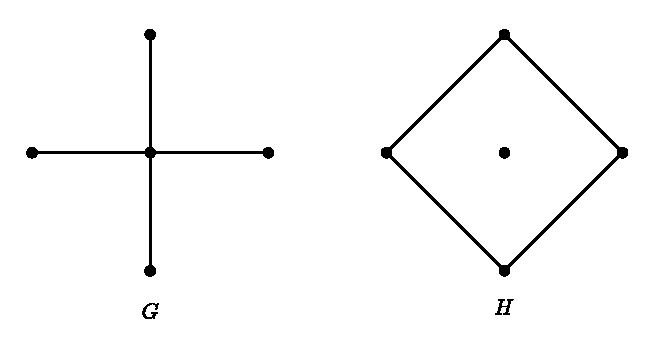
\includegraphics{images/isospektral}
  \caption{Zwei nicht isomorphe Graphen}
  \label{fig:isospektralgraphen}
\end{figure}
Lemma \ref{lem:GraphEigenwerte} impliziert insbesondere, dass isomorphe Graphen dasselbe charakteristische Polynom und somit dasselbe Spetkrum haben. Die Umkehrung gilt hingegen nicht. Dazu betrachten wir die Graphen $G$ und $H$, wobei $G=K_{1,4}$ ein Stern ist und $H=C_4+K_1$, die disjunkte Vereinigung von $C_4$ und $K_1$ ist (siehe Abbildung \ref{fig:isospektralgraphen}).
\todo{Bild neu} Diese sind offenbar nicht isomorph. Wir k"onnen die Ecken so nummerieren, dass f"ur die Adjazenzmatrizen gilt: 
\begin{align*}
  A(G) = \begin{pmatrix}
    0 & 1 & 1 & 1 & 1 \\
    1 & 0 & 0 & 0 & 0 \\
    1 & 0 & 0 & 0 & 0 \\
    1 & 0 & 0 & 0 & 0 \\
    1 & 0 & 0 & 0 & 0 
  \end{pmatrix}  \text{ und }A(H) = \begin{pmatrix}
    0 & 0 & 0 & 0 & 0 \\
    0 & 0 & 1 & 0 & 1 \\
    0 & 1 & 0 & 1 & 0 \\
    0 & 0 & 1 & 0 & 1 \\
    0 & 1 & 0 & 1 & 0 
  \end{pmatrix}
\end{align*}
Eine einfache Rechnung liefert dann $$p_G(\lambda) = p_H(\lambda) = -\lambda^{3}(\lambda+2)(\lambda-2)$$ und somit 
$$\operatorname{sp}(G)=\operatorname{sp}(H) = (2,0,0,0,-2).$$
Die Graphen $G$ und $H$ haben dasselbe Spektrum, sind aber nicht isomorph.
Zwei Graphen hei{\ss}en \DF{isospektral}, falls sie das selbe Spektrum besitzen. Isomoprhe Graphen sind also stets isospektral, aber nicht umgekehrt. 

Die Graphentheorie besch"aftigt sich mit der Struktur und den Eigenschaften von Graphen. Eine \DF{Grapheneigenschaft} ist eine Klasse von Graphen, die mit jedem Graphen $G$ auch alle dazu isomorphen Graphen enth"alt. So ist zum Beispiel Zusammenhang (d.h. die Klasse der zusammenh"angenden Graphen) eine Grapheneigenschaft. Eine \DF{Spektraleigenschaft von Graphen} ist eine Klasse von Graphen, die mit jedem Graphen $G$ auch alle dazu isospektralen Graphen
enth"alt. 
Dann ist jede Spektraleigenschaft von Graphen auch eine Grapheneigenschaft, aber nicht umgekehrt. Wie das obige Beispiel isospektraler Graphen $K_{1,4}$ und $C_4+K_1$ zeigt, ist Zusammenhang keine Spektraleigenschaft. 
\subsection{Eigenschaften des Graphenspektrums}
In diesem Abschnitt wollen wir einige einfache, aber wichtigen Eigenschaften der Spektra von Graphen anf"uhren.
Eine Matrix $A\in\Rnn$ hei�t \DF{reduzibel}, falls zwei nichtleere disjunkte Teilmengen $X,Y$ von $\{ 1,\dots,n \}$ existieren, mit $X\cup Y = \{ 1,\dots,n \}$ und $$A_{ik} = 0 ~ i\in X, k \in Y,$$ anderfalls hei�t $A$ \DF{irreduzibel}. 
Wie man leicht zeigen kann, ist $A$ genau dann reduzibel, wenn man $A$ durch Umordnen der Zeilen und Spalten in folgende Blockform "uberf"uhren kann: $$\begin{pmatrix}
  A_{11} & 0 \\ A_{12} & A_{22}
\end{pmatrix}.$$ 
Ist $G$ ein Graph, so gilt $$G \text{ ist zusammenh"angend} \Leftrightarrow A(G) \text{ ist irreduzibel}.$$
Anfang des vorherigen Jahrhunderts besch"aftigten sich Perron \cite{Perron07} und Frobenius \cite{Frobenius12} mit dem Spektrum von unzerlegbaren Matrizen mit nicht negativen Elementen, insbesondere mit dem \DF{Spektralradius} solcher Matrizen, d.h., ihrem betragsm"a�ig gr"o�tem Eigenwert. Die von ihnen erzielten Ergbnisse, welche als Satz von Perron-Frobenius bekannt sind, spielen in vielen Teilgebieten der Mathematik (Analysis, Numerik, Stochastik, Graphentheorie usw.) eine wichtige Rolle. Der folgende
Satz ist ein unmittelbare Folgerung aus dem Satz von Perron-Frobenius.

\begin{theorem}
  F"ur einen zusammenh"angenden Graphen $G$ der Ordnung $n\in \N$ gelten folgende Aussagen:
  \begin{enumerate}[label=\rm{(\alph*)}]
    \item $\lambda_{max}(G)$ ist ein einfacher Eigenwert mit $\lambda_{max}(G) \leq \Delta(G)$.
    \item Es gibt einen Eigenvektor $x$ von $G$ zum Eigenwert $\lambda_{max}(G)$ mit $x(v) > 0$ f"ur alle $v\in V(G)$. 
    \item Ist $x$ ein Eigenvektor von $G$ zum Eigenwert $\lambda$ mit $x(v)> 0$ f"ur alle $v\in V(G)$, so ist $\lambda = \lambda_{max}(G)$.
    \item F"ur alle Eigenwerte $\lambda$ von $G$ gilt $|\lambda| \leq \lambda_{max}(G)$.
  \end{enumerate}
\end{theorem}

\begin{corollary}
  F"ur einen $r$-regul"aren Graphen $G$ der Ordnung $n \in\N$ gelten folgende Aussagen:
  \begin{enumerate}[label=\rm{(\alph*)}]
    \item $\lambda_{max}(G) = r$.
    \item $G$ ist genau dann zusammenh"angend, wenn $\lambda_{max}(G)$ ein einfacher Eigenwert ist.
  \end{enumerate}
  \label{cor:regulargrapheigenvalue}
\end{corollary}

\begin{proof}
  Es seien $G_1,\dots,G_l$ die Komponenten von $G$. Dann ist jede Komponente $G_i$ ein $r$-regul"arer Graph ($1\leq i \leq l$). Damit folgt aus (\ref{eq:Grregul}), dass $\mathbbm 1$ ein Eigenvektor von $G_i$ zum Eigenwert $r$ ist. Dann ist $\lambda_{max}(G) = r$ und $m_{G}(r) = l$. Daraus folgt dann sowohl (a) als auch (b).
\end{proof}

\begin{corollary}
  Ist $G$ ein $r$-regul"arer Graph der Ordnung $n\geq 1$, so gelten folgende Aussagen:
  \begin{enumerate}[label=\rm{(\alph*)}]
    \item $\lambda_{1}(G) = r $ und $\lambda_{1}(\overline{G}) = n-1-r $.
    \item $\lambda_{i}(\overline{G}) = - \lambda_{n-i+1}(G) -1$ f"ur $2\leq i \leq n$. 
  \end{enumerate}
\end{corollary}

\begin{proof}
  Aussage (a) folgt aus Korollar \ref{cor:regulargrapheigenvalue}, da der Komplementargraph eines $r$-regul"aren Graphen $(n-1-r)$-regul"ar ist. 
  Zum Beweis von (b) w"ahlen wir f"ur $G$ und $\overline{G}$ die selbe Nummerierung der Ecken. Dann ist $$A(G) + A(\overline{G}) = J-I$$ wobei $J \in \Rnn$ die $1$-Matrix ist, und $I\in\Rnn$ die Einheitsmatrix ist. Wir betrachten $\lambda = \lambda_i(G)$ f"ur $i \geq 2$. Dann existiert ein Eigenvektor $x$ zum Eigenwert $\lambda$. Dieser ist orthogonal zu $\mathbbm 1 \in E_{G}(r)$. Folglich ist 
  \begin{align*}
    A(G)x + A(\overline{G})x = Jx -Ix = -x
  \end{align*}
  Durch Umstellen erhalten wir $A(\overline{G})x = (-\lambda-1)x$. Also ist $(-\lambda-1)$ ein Eigenwert von $\overline{G}$. Analog k"onnen wir zeigen, dass f"ur $\lambda = \lambda_{i}(\overline{G})$  ($i\geq 2$) $-1-\lambda$ ein Eigenwert von $G$ ist. 
\end{proof}

\begin{lemma}
  \label{lem:evGraph} 

  Sei $G$ ein Graph der Ordnung $n\in\N$ mit $m$ Kanten. Dann gilt:
  \begin{enumerate}[label={\rm(\alph*)}]
    \item $\lambda_{1}(G) + \lambda_{2}(G) + \dots + \lambda_{n}(G) = 0$.
    \item $\lambda_{1}(G)^{2} + \lambda_{2}(G)^{2} + \dots + \lambda_{n}(G)^{2} = 2m$.
  \end{enumerate}
\end{lemma}

\begin{proof}
  Wir zeigen zun"achst (a). F"ur die Adjazenzmatrix $A = A(G)$ gilt $\operatorname{spur}(A)  = \sum\limits_{i=1}^{n} a_{ii}= 0$. Aus der Linearen Algebra ist bekannt, dass $\sum\limits_{i=1}^{n}\lambda_{i}(A) = \operatorname{spur}(A) = 0$ ist.  

  Um (b) zu beweisen, betrachten wir $B=A^{2}$. Die Eintr"age $B_{ij}$ geben die Anzahl aller Kantenfolgen der L"ange $2$ zwischen den Ecken $v_i$ und $v_j$ an. Insbesondere gilt $B_{ii} = d_{G}(v_i)$, da jede Kantenfolge der L"ange $2$ von $v_i$ nach $v_i$ genau einer Kante entspricht. Daraus folgt:

  \begin{equation*}
    \sum\limits_{i=1}^{n} \lambda_{i}(G) ^{2} = \operatorname{spur}(B) = \sum\limits_{i=1}^{n} B_{ii} =  \sum\limits_{i=1}^{n} d_{G}(v_{i}) = 2m.
  \end{equation*}
  Somit gilt (b).
\end{proof}

\begin{lemma}
  Seien $H$ ein induzierter Untergraph von $G$ und $k = |G| - |H|$. Dann gilt
  $$ \lambda_p(G) \geq \lambda_{p}(H) \geq \lambda_{p+k}(G)$$
  f"ur $1\leq p \leq n-k$.
  \label{lem:InterlacingGraphen}
\end{lemma}

\begin{proof}
  Ist $H$ ein induzierter Untergraph von $G$, so entsteht $A(H)$ aus $A(G)$ durch Streichen von Spalten und den korrespondierenden Zeilen. Damit folgt die Behauptung aus Satz \ref{thm:Interlacing}.
\end{proof}

\begin{corollary}
  Sei $G$ ein Graph mit $\omega(G) = p$ und $\alpha(G) = q$. Dann gilt:
  $$ \lambda_p(G) \geq -1 \mbox{ und } \lambda_q(G) \geq 0 \text{.} $$
  \label{cor:alphaomegaEigenwerte}
\end{corollary}
\begin{proof}
  Ist $\omega(G) = p$, so besitzt $G$ einen vollst"andigen induzierten Untergraphen $H$, der Ordnung $p$. Dann gilt $\lambda_{1}(H) = p-1$ und $\lambda_{i}(H) = -1$ f"ur $2\leq i \leq p$(siehe Beispiel \ref{ex:vollstgraph}). Damit folgt aus Korollar \ref{lem:InterlacingGraphen}, dass $\lambda_{p}(G) \geq \lambda_{p}(H) \geq -1$ ist.  
  Ist $\alpha(G) = q$, so besitzt $G$ einen kantenlosen induzierten Untergraphen $H'$ der Ordnung $q$.
  Dann ist $\lambda_{i} (H') = 0$ f"ur  $1\leq i \leq q$. Also folgt aus Korollar \ref{lem:InterlacingGraphen}, dass $\lambda_{q}(G) \geq \lambda_{q}(H') = 0$ ist.
\end{proof}

Wir wollen uns nun noch kurz mit den Eigenwerten von Kantengraphen befassen. Es sei $G=L(H)$ der Kantengraph des Graphs $H$ mit $V(H) = \{v_1,v_2,\dots,v_n\}$ und $E(H) = \{e_1,e_2,\dots,e_m\}$. Wir betrachten die Inzidenzmatrix $B=B(H) \in \R^{n\times m}$ mit 
$$B_ij = \begin{cases}
  1 & \text{ falls } v_i \in e_j \\
  0 & \text{ falls } v_i \notin e_j . \\
\end{cases}$$
Dann erhalten wir die folgenden Beziehungen:
$$A(G) = B^{T}B -2I \text{ und } A(H) = BB^{T} - D,$$
wobei $D= \operatorname{diag}(d_H(v_1),d_H(v_2),\dots,d_H(v_n)$ die Gradmatrix von $H$ ist. Die Matrizen $B^{T}B$ und $BB^{T}$ sind dann positiv semidefinit und folglich sind ihre Eigenwerte nicht negativ (siehe Satz \ref{prop:psdmatrix}). 
F"ur den $p$-gr"o{\ss}ten Eigenwert von $G$ gilt somit 
$$ \lambda_{p}(G) = \lambda_{p}(B^{T}B) -2 \geq -2,$$ also ist insbesondere $\lambda_{min}(G) \geq -2$. 
Ist der Graph $H$ kreislos, und damit ein Wald, so ist $\operatorname{rang}(B) = m$ \todo{einheitlicher rang} (wie sich leicht durch Induktion nach $n$ zeigen l"asst). Dann ist $B^{T}B$ positiv definit und somit $\lambda_{min}(G) > -2$. 
Zusammenfassend erhalten wir dann folgendes, wohlbekanntes Resultat (siehe \cite[Theorem 6.11]{CvetkovicDS79}).

\begin{theorem}
  Ist $G=L(H)$ der Kantengraph eines Graphen $H$, so ist $\lambda_{min}(G) \geq -2$. Ist $H$ ein Wald, so ist $\lambda_{min}(G) > -2$. 
  \label{cor:linegraphwald}
\end{theorem}
Aus der Linearen Algebra wei{\ss} man, dass die Matrizen $BB^{T}$ und $B^{T}B$ dieselben Eigenwerte mit den selben Vielfachheiten besitzen, mit Ausnahme des Eigenwerts $\lambda = 0$. Es gilt dann
$$ \lambda^{n} p_{B^{T}B} (\lambda) = \lambda^{m} p_{BB^{T}} (\lambda)$$
Die Vielfachheit des Eigenwerts $\lambda = 0$ h"angt nur von dem Rang der Matrix $B$ ab. Ist $H$ zusammenh"angend und $n\geq 2$, so kann der Rang von $B$ nur die Werte $n$ oder $n-1$ annehmen, je nachdem ob $H$ bipartit ist oder nicht. Dies wurde zuerst von Sachs \cite{Sachs} gezeigt. 
Daraus erh"alt man folgendes Resultat (siehe auch das Buch von Cvetkovi\'c, Rowlinson und Simi\'c \cite[Theorem 2.2.4]{CvetkovicRowSlob10}.

\begin{theorem}
  Es sei $H$ ein zusammenh"angender Graph mit $n$ Ecken und $m$ Kanten, wobei $n\geq 2$ ist. F"ur die Vielfachheit des Eigenwertes $\lambda = -2$ von $G=L(H)$ gilt:
  $$m_G(-2) = \begin{cases}
    m-n+1 &\text{ falls } H \text{ bipartit ist} \\
    m-n &\text{ sonst.}
  \end{cases}$$
  \label{thm:sachszshgrapheigenwert}
\end{theorem}

In den 1970er Jahren sind verschieden Arten erschienen, die sich mit der Charakterisierung der Graphen $G$ mit $\lambda_{min}(G) \geq -2$ befassen.
Zur Geschichte dieses Problems siehe \cite{CvetkovicRowSlob10}.
Eine erste Teilcharakterisierung dieser Graphenklasse wurde 1977 von Hoffman \cite{Hoffman77}, eine vollst"andige Charakterisierung wurde 1978 von Cameron, Goethals, Seidel und Shult \cite{CameronGSS78} gefunden.
